\documentclass[a4paper, 11pt]{article}
\usepackage{comment} % enables the use of multi-line comments (\ifx \fi) 
\usepackage{lipsum} %This package just generates Lorem Ipsum filler text. 
\usepackage{fullpage} % changes the margin
\usepackage{libertine}
\usepackage{color}
\usepackage[braket, qm]{qcircuit}
\usepackage{amssymb}
\usepackage{amsmath}
\usepackage{pgf,tikz}
\usepackage{graphicx}
\usetikzlibrary{automata, positioning}
\usetikzlibrary{shapes,arrows}
\newtheorem{definition}{Definition}
\newtheorem{example}{Example}
\newcommand{\nevComment}[1]{\textcolor{red}{RN: #1}}
\newcommand{\roothalf}{\frac{1}{\sqrt{2}}}
\newcommand{\half}{\frac{1}{2}}
\newcommand{\hrh}{\frac{1}{2\sqrt{2}}}
\linespread{1.1}

\begin{document}
\title{Quantum Systems as Coalgebras}
\author{Luis S. Barbosa \and Liu Ai \and Renato Neves}
\maketitle

\section{Introduction}

\subsection{Quantum computing}

In the recent hundred of years, quantum mechanics fundamentally changed human understanding of structures and interactions of materials. Quantum mechanics has been applied in many natural sciences, such as the structure of the atom, nuclear fusion in stars, the structure of DNA, etc. On the other hand, we can take advantage of quantum features to provide powerful models of computation in formal sciences, especially in theoretical computer science. Quantum computing rose in response to the proper time and conditions. 

Quantum computing has many advantages worth learning. Firstly, quantum computing provides a method of bypassing the end of Moore's Law. Secondly, there are certain problems that can be solved more efficiently by quantum computing than  any classical computational method. A few examples can be found in \cite{NM08}. Thirdly, quantum computing allows us to break classical cryptography schemas, which is demonstrated in quantum information \cite{nielsen2002quantum}. Moreover, there are other compelling advantages, such as quantum programming \cite{ying16}.

In aforementioned documents, a quantum system is built on a Hilbert space. At a fixed time, states and observables can give a full description of a quantum system. There are two representations of states: vectors in the corresponding Hilbert space and density matrices, which are the matrix representations of density operators over the corresponding Hilbert space with unit trace . Vectors can only represent pure states, while density matrices can represent pure states and mixed states. Observables are the physical quantities that can be observed in each state. Observables are often represented by self-adjoint mappings, whose matrix representations are Hermitian matrices. 

The static descriptions of a quantum system are not enough for quantum computing. We also need to know the dynamics of a quantum system, i.e., how a quantum system changes in time. For vector states in a closed quantum system, the dynamics are given by unitary operators, which preserve the unit trice. If a quantum system is open, measurements or projections should be considered in the dynamics. In reality, no quantum system is completely isolated from its environment, thus every quantum system is open to some extent. 


\nevComment{\underline{Goal of this subsection}: To convince the
  reader of the importance of quantum computing, and to give a first
  introduction to quantum systems.  \underline{Useful references}:
  \cite{nielsen2002quantum,NM08,ying16}. }


\subsection{Objectives}

The goals of the present work are,
\begin{enumerate}
\item to provide a unifying view of the
  current models for quantum transition systems;
\item and to formally relate them in terms of expressivity.
\end{enumerate}
\nevComment{We need to explain why these objectives are relevant.
  Note that subsequently we will use them to provide uniform, useful
  notions to quantum transition systems. Which notions for
  such systems are useful is still a matter of
  discussion.}

\subsection{What coalgebras bring into the game}

Coalgebras, as pairs $\langle S,\alpha:S\rightarrow FS\rangle$ for a functor $F$, are an elegant generalization of transition systems. A coalgebra consists of a state space $S$ and a map $\alpha$, which captures the possible outcomes and the dynamics of the structure decided by $F$. A transition system consists of states and transitions between states, which can be  simulated by a map with a certain functor. Coalgebras can thus describe general transition systems provided with transitions whose structure given by certain functor. There are many classical examples in \cite{rutten2000}. 

Coalgebras provide a uniform way of treating transitions system by general notions and results \cite{Jacobs16}. For instance, one of the fundamental notions is bisimilarity, which indicates two internally different states are indistinguishable as far as one can see with the available operations and corresponds to the notion of bisimulation in transition systems. Moreover, there are some general properties of states, such as invariant and safety. Coalgebraic analysis can also help us to consider expressiveness and the hierarchy of different types of systems.

There is an overview of some existing insights in the theory of coalgebras in \cite{rutten2000}. Besides, many types of dynamic systems are described by different functors, such as deterministic and non-deterministic systems, Mealy and Moore machines, and so on.  Coalgebraic analysis can also be applied to more complicated systems, like probabilistic systems and hybrid systems. The theory of coalgebras is used to conduct a detailed comparative study of different probabilistic transition systems \cite{sokolova}.  A coalgebraic perspective provides a generic theory of hybrid automata with abundant notions and compelling results \cite{neves17}. 

\nevComment{\underline{Goal of this subsection}: To tell the reader in
  which ways coalgebras can help better understand transition systems
  and develop tools for their analysis.  We will need to explain that
  coalgebras are a very useful framework for providing
  uniform views of (apparently) different types of transition
  systems. \underline{Useful references}:
  \cite{rutten2000,Jacobs16,sokolova,neves17}. }

\subsection{Document structure and notation}

\nevComment{\underline{Goal of this subsection}: To guide the reader
  along the document so that he can get a broad picture of our
  exposition at an early stage. Setting (non-standard) notation at a
  common point is also useful to the reader, since he then knows where
  to look when unfamiliar notation appears.}

\section{A Primer on Quantum Computing}

\subsection{What makes it different from classical paradigms}

In quantum world, the uncertain principle, which says that certain properties of particles just cannot be known, brings about challenges for computational models. Versions of double-slit experiments suggest that a microscopic object, like a photon, can be in many positions at the same time, a superposition, and that observation can change the nature of subatomic particles \cite{NM08}. We see a particle in a certain position because a measurement has been performed. After measuring a quantum object, it is no longer be in a superposition.     

Different from most other branches of sciences, quantum computing is based on complex numbers. Due to the appearance of superposition, sets do not have good compatibility in being the state spaces of quantum systems. In order to capture these features of the quantum world, most formalisms for quantum systems are built on complex Hilbert spaces. Below we introduce some notions for Hilbert spaces \cite{hirvensalo11,G08}.

We can understand an n-dimensional Hilbert space $H_n$ as the complex vector space $\mathbb{C}^n$ equipped with Hermitian inner product $\langle \boldsymbol{x}|\boldsymbol{y}\rangle=\overline{x_1}y_1+\cdots+\overline{x_n}y_n$, where $\overline{z}$ is the conjugate of $z$. The norm induced by Hermitian inner product is $\|\boldsymbol{x}\|=\sqrt{\langle\boldsymbol{x}|\boldsymbol{x}\rangle}$. Given an $\boldsymbol{x}=(x_1,\dots,x_n)\in H_n$, we define $\ket{\boldsymbol{x}}$ (called ket-vector) to be a column vector $(x_1,\dots,x_n)^T$ (the transpose of $(x_1,\cdots,x_n)$) and $\bra{\boldsymbol{x}}$ (called bra-vector) to be a row vector $(\overline{x_1},\dots,\overline{x_n})$. Kets are also called state vectors, describing only pure states of quantum systems. In most cases, unit state vectors are picked.  A superposition can be represented by a pure state, which has the form of $\ket{\phi}=\alpha_1\ket{\phi_1}+\cdots+\alpha_n\ket{\phi_n}$ satisfying $|\alpha_1|^2+\cdots+|\alpha_n|^2=1$ for a given basis $\phi_1,\dots,\phi_n$ of $H_n$.

\begin{definition}
The set of all bounded linear operators from a Hilbert space $H$ is denoted by $B(H)$.  An operator $A\in B(H)$ is called 
\begin{itemize}
\item[(a)] normal if $AA^*=A^*A$, where $A^*$ is the conjugate transpose of $A$.
\item[(b)] self-adjoint if $A=A^*$.
\item[(c)] positive if\ \ $\forall x\in H,\langle Ax,x\rangle\ge 0$.
\item[(d)] unitary if $A^*A=AA^*=I$.
\item[(e)] idempotent $A=A^2$.
\item[(f)] projection if $A=A^2=A^*$, i.e., A is both self-adjoint and idempotent. 
\item[(g)] density if A is a self-adjoint positive operator with unit trace. 
\end{itemize}
\end{definition}

Density matrices, representations of density operators, can describe both pure and mixed states. The density matrix is obtained from the density operator by choice of basis in the underlying space. Naturally, density matrices are self-adjoint positive matrices with unit trace. The set of all density matrices of a Hilbert space is denoted by $\mathcal{DM}(H)$.  An observable of a quantum system is a self-adjoint operator. An effect is a positive operator $A$ satisfying $I-A$ is also positive and the set of all effects over $H$ is denoted by $\mathcal{E}f(H)$. A linear mapping from $\phi:B(H_1)\rightarrow B(H_2)$ is called positive if $\phi(A)$ is positive for all positive $A$. A linear mapping from $\phi:B(H_1)\rightarrow B(H_2)$ is called completely positive if $\phi\otimes I$ is a positive mapping in $H_1\otimes K\rightarrow H_2\otimes K$, where $I$ is an identity mapping on any complex Hilbert space $K$ and $\otimes$ represents tensor product \cite{NM08}. A quantum operation ($QO$) from an m-level quantum system to an n-level quantum system is a complete positive linear mapping $\mathcal{E}:\mathcal{DM}(H_m)\rightarrow \mathcal{DM}(H_n)$, satisfying trace condition:
$$
\frac{\texttt{tr}(\mathcal{E}(\rho))}{\texttt{tr}(\rho)}\in [0,1]\  for\ any\ \rho\in \mathcal{DM}(H_m)\ such \ that\ \texttt{tr}(\rho)>0
$$ 
Especially, if $\texttt{tr}(\mathcal{E}(\rho))=\texttt{tr}(\rho)$, we call $\mathcal{E}$ trace-preserving. The set of all quantum operations from an m-level quantum system to an n-level quantum system is denoted by $QO_{m,n}$. When a quantum operation $\mathcal{E}$ satisfies $\mathcal{E}(\rho)=\sum_i E_i\rho E_i^*$ for some $n\times m$ matrices $(E_i)$, we use the notation by denotation $\mathcal{E}=\{E_i\}$.

\nevComment{\underline{Goal of this subsection}: To explain to the
  reader why quantum computing is a challenging thing, and why the
  problems that we are addressing are non-trivial. References from
  subsection 1.1 can also be used here.  Emphasise the problem of
  superposition and observation. We set the basic machinery of quantum
  computing (\emph{e.g.} Hilbert spaces, unitary matrices) in this subsection.}

\subsection{A general view of its current formalisms}

Research on quantum computing has been developed for many years and different formalisms have emerged. Besides that transition systems are suitable for capturing quantum states and transformations between them, there are other compelling formalisms from different perspectives as follows.
\begin{itemize} 
\item When it comes to realizing the concept of superposition, the notion of qubit is inevitable. A quantum circuit is a model where a quantum computation is a sequence of quantum gates, which are reversible transformations on an n-qubit register \cite{nielsen2002quantum, NM08}. The circuit model for quantum computing has a new representation by building quantum gates as ZX-diagrams in quantum picturalism, which is about how to glue the development of the diagrammatic language and the presentation of quantum theory as a process theory. Quantum picturalism is rich enough to discuss quantum features and provides a intuitive and diagrammatic description for quantum computing \cite{BA17}.  
\item Useful quantum algorithms must eventually be realized in concrete software by quantum programming \cite{ying16}. Quantum circuits emphasize data flow, while quantum programming can express both data flow and control flow. Quantum programming languages can also capture high-level features and high-order computation \cite{selinger04,hasuo17}.
\item Quantum computing and quantum communication are two important branches in quantum information science. Process algebras provide a tool for the high-level description of interactions, communications, and synchronizations between processes. Quantum process algebras allow us to integral quantum computing and quantum communication \cite{jorrand04,ying09}. They also provide algebraic laws that allow process descriptions to be manipulated and formal techniques for  analysis and verification. 
\end{itemize}

\nevComment{\underline{Goal of this subsection}: To give the reader a
  broad view of what is currently being done in regard to semantics of
  quantum systems. This includes not only transition systems, but also
  programming languages \cite{selinger04,hasuo17,ying16}, circuit
  formalisms \cite{nielsen2002quantum}, and process algebras
  \cite{jorrand04,ying09}. In the following sections our focus will be
  mainly on transition systems.}

\subsection{Examples of quantum systems}
Here we list some examples of quantum systems to be used for illustrating different formalisms of quantum transition systems. 

\begin{example}(quantum random walk)
\label{QRW}
A quantum Markov chain is a triple $(H,\mathcal{E},\phi)$ where $H$ is a Hilbert space, $\mathcal{E}$ is a quantum operator over $H$ to describe how the random walk moves at each step and $\phi$ is the initial vector state over $H$. Quantum random walk is a special case of quantum Markov chains, where 
$$\begin{aligned}
H&=\{\sum_{i}d_i\ket{\downarrow}\otimes\ket{i}+u_i\ket{\uparrow}\otimes\ket{i}\ |i\in \mathbb{Z}\ and\ c_i,u_i\in \mathbb{C}\}\\
\mathcal{E}&(\ket{\uparrow}\otimes\ket{i})=\roothalf\ket{\uparrow}\otimes\ket{i-1}+\roothalf\ket{\downarrow}\otimes\ket{i+1}\\
\mathcal{E}&(\ket{\downarrow}\otimes\ket{i})=\roothalf\ket{\uparrow}\otimes\ket{i-1}-\roothalf\ket{\downarrow}\otimes\ket{i+1}
\end{aligned},
$$
$\ket{i}$ as the position of the particle, $\ket{\downarrow}$ and $\ket{\uparrow}$, respectively, as the left direction and right direction of the walk. 

Given a start state $\ket{\uparrow}\otimes\ket{0}$ and after one step we have:
$$\mathcal{E}(\ket{\uparrow}\otimes\ket{0})=\roothalf\ket{\uparrow}\otimes\ket{-1}+\roothalf\ket{\downarrow}\otimes\ket{1}.$$
After two steps we get:
$$\mathcal{E}^2(\ket{\uparrow}\otimes\ket{0})=\half\ket{\uparrow}\otimes\ket{-2}+\half(\ket{\uparrow}+\ket{\downarrow})\otimes\ket{0}-\half\ket{\downarrow}\otimes\ket{2}.$$
After three steps we get:
$$
\mathcal{E}^3(\ket{\uparrow}\otimes\ket{0})=\hrh\ket{\uparrow}\otimes\ket{-3}+\roothalf\ket{\uparrow}\otimes\ket{-1}+\hrh\ket{\downarrow}\otimes\ket{-1}-\hrh\ket{\uparrow}\otimes\ket{1}+\hrh\ket{\downarrow}\otimes\ket{3}.
$$
Note that the probability of seeing $\ket{-1}$ as outcome is more than the probability of seeing $\ket{1}$ as outcome, which determined by the unitary operator $\mathcal{E}$.
\end{example}

\begin{example}
 \label{QA}
 There is a quantum version of finite automata, where states are vector states in a Hilbert space, the transition matrix is unitary for an given input and the output is decided by the measurement. The following state diagram is an example of a quantum automaton over the input set $A={a,b}$ and the state space $\mathbb{C}^2$ with the standard basis $\ket{0},\ket{1}$. 
\begin{center}
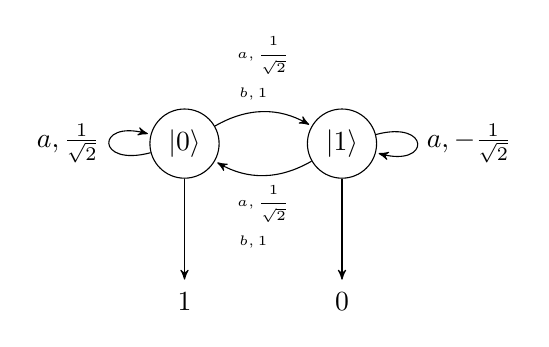
\begin{tikzpicture}[shorten >=1pt,node distance=2cm,on grid,>=stealth']
\node[state] (x_0) {$\ket{0}$};
\node[state] (x_1)  [right=of x_0] {$\ket{1}$};
\node (y_0) [below=of x_0] {1};
\node (y_1) [below=of x_1] {0};
\path[->] (x_0) edge[bend left] node (a_0) [above] {\tiny{$\begin{aligned}a&,\roothalf\\b&,1 \end{aligned}$}}  (x_1)
(x_1) edge[bend left] node [below ] {\tiny{$\begin{aligned}a&,\roothalf\\b&,1 \end{aligned}$}} (x_0)
(x_0) edge (y_0)
(x_1) edge (y_1)
(x_0) edge [loop left] node {$a,\roothalf$} ()
(x_1) edge [loop right] node {$a,-\roothalf$} ();
\end{tikzpicture}
\end{center} 
The transition matrices are
$$
T_a=\roothalf\begin{bmatrix}
1&1 \\
1&-1
\end{bmatrix}, 
T_b=\begin{bmatrix}
0&1\\
1&0
\end{bmatrix}.
$$
The outcomes of states are the probabilities to see $\ket{0}$. Given the initial state $\ket{0}$, the above automaton gives a probabilistic language $\{a,b\}^*\rightarrow[0,1].$ For instance, the probability that the word $ba$ is accepted  is $\half$. 
\end{example}


\begin{example}(quantum teleportation protocol]
\label{QTP}
\[
\Qcircuit @C=.7em @R=.4em @! {
\lstick{C: \ket{\psi}} & \qw & \qw & \ctrl{1} & \gate{H} & \meter & \control \cw\\
\lstick{A: \ket{0}} & \qw & \targ & \targ & \qw & \meter & \cwx\\
\lstick{B: \ket{0}} & \gate{H} & \ctrl{-1} & \qw & \qw & \gate{X} \cwx & \gate{Z} \cwx & \rstick{\ket{\psi}} \qw
}
\]
Above picture is the quantum circuit for quantum teleportation protocol, where $H$ is a Hadamard matrix, $X,Z$ are respectively the Pauli-$X$ matrix and the Pauli-$Z$ matrix. The  protocol is then as follows:
\begin{itemize}
\item[1.] The teleportation protocol begins with a quantum state $\ket{\psi}$, in Alice's possession, that she wants to convey to Bob. This qubit can be written as $$\ket{\psi}_C=\alpha\ket{0}_C+\beta\ket{1}_C, \alpha,\beta\in \mathbb{C}\ and\ |\alpha|^2+|\beta|^2=1.$$
The subscript C above is used only to distinguish this state from below $A$ and $B$.
\item[2.] Next, the protocol requires that Alice and Bob share a maximally entangled state, which is picked as $\Phi^+_{AB}=\roothalf(\ket{0}_A\otimes\ket{0}_B+\ket{1}_A\otimes\ket{1}_B)$ here.
\item[3.]The total three particle state, of $A$, $B$ and $C$ together, thus becomes the following four-term superposition:
$$
\begin{aligned}
\ket{\psi}_C\otimes \ket{\Phi^+}_{AB}=&\half[\ket{\Phi^+}_{AC}\otimes(\alpha\ket{0}_B+\beta\ket{1}_B)+\ket{\Phi^-}_{AC}\otimes(\alpha\ket{0}_B-\beta\ket{1}_B)\\
&+\ket{\Psi^+}_{AC}\otimes(\beta\ket{0}_B+\alpha\ket{1}_B)+\ket{\Psi^-}_{AC}\otimes(\beta\ket{0}_B-\alpha\ket{1}_B)]. 
\end{aligned}$$
\item[4.] After Bob receives the result from Alice's Bell measurements, he performs a unitary operation on his particle to transform it to the desired state $\alpha\ket{0}_B+\beta\ket{1}_B$:
\begin{itemize}
\item If the result is $\ket{\Phi^+}_{AC}$, Bob knows his qubit is already in the desired state and does nothing, which means the identity operator.
\item If the result is $\ket{\Phi^-}_{AC}$, Bob would send his qubit through the unitary quantum gate given by the Pauli-$X$ matrix $X=\begin{bmatrix}
1 & 0\\
0 & -1
\end{bmatrix}.$
\item If the result is $\ket{\Psi^+}_{AC}$, Bob would send his qubit through the unitary quantum gate given by the unitary quantum gate given by the Pauli-$Z$ matrix $Z=\begin{bmatrix} 0 & 1\\1 & 0\end{bmatrix}.$
\item If the result is $\ket{\Psi^-}_{AC}$, Bob would send his qubit through the unitary quantum gate given by the composition $X\circ Z=\begin{bmatrix}  0 & 1\\ -1 & 0\end{bmatrix}.$ 
\end{itemize}
\end{itemize}
\end{example}





\nevComment{\underline{Goal of this subsection}: To introduce the
  reader to a stock of examples of quantum systems. They will be used
  for illustrating different formalisms of quantum transition
  systems. \emph{N.b.}: in subsequent work we will also use them as
  guiding principles for developing new models of quantum systems.}

\section{A Primer on Coalgebra}
In the sequel we introduce some basic notions in coalgebra theory \cite{rutten2000,Jacobs16} and present a couple of results of coalgebraic analysis of probabilistic systems \cite{sokolova}.

\subsection{Basic notions}
A \textbf{category} comprises objects and arrows, where objects are linked by arrows. A category satisfies two basic requirements: the ability to compose the arrows associatively and the existence of an identity arrow for each object. \textbf{Set} is the category of sets, whose objects are sets and arrows are functions.  \textbf{Conv} is the category of convex sets, whose objects are convex sets and arrows are convex maps, which preserve all convex combinations. 

A functor $F$ from $C$ to $D$ is a mapping preserving identity morphisms and composition of morphisms. An endofunctor $F$ on a certain category is a functor from the category to itself. Let $F$ be an endofunctor on a certain category. An $F$-coalgebra or $F$-system over the category is a pair $(S,\alpha_S)$ consisting of an object $S$ in the category and a mapping $\alpha_S:S\rightarrow F(S)$. The object $S$ is called the carrier of the system,  also called the state space. The mapping $\alpha_S$ is called the $F$-transition structure (or dynamics) of the system. For instance, given the identity functor $\mathcal{I}$ and the power set functor $\mathcal{P}$ on \textbf{Sets}, an $\mathcal{I}$-coalgebra $(S,\alpha_S:S\rightarrow \mathcal{I}(S))$ corresponds to a deterministic system and a $\mathcal{P}$-coalgebra $(S,\alpha_S:S\rightarrow \mathcal{P}(S))$ corresponds to a nondeterministic system.

Let $(S,\alpha_S)$ and $(T,\alpha_T)$ be two $F$-coalgebras, where $F$ is an arbitrary functor on a certain category. A function $f:S\rightarrow T$ is a $F$-homomorphism, if $F(f)\circ \alpha_S=\alpha_T\circ f$:
\begin{center}
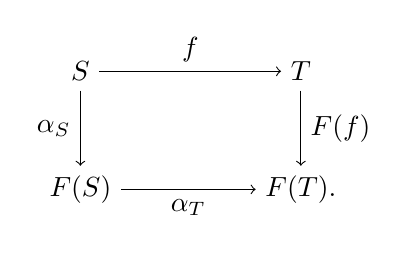
\begin{tikzpicture}
\node[fill=white] (a) at (0,0) {$S$};
\node[fill=white] (b) at (2.8,0) {$T$};
\node[fill=white] (c) at (0,-1.5) {$F(S)$};
\node[fill=white] (d) at (2.8,-1.5) {$F(T).$};
\draw[->] (a) to node [above]{$f$} (b);
\draw[->] (a) to node [left]{$\alpha_S$} (c);
\draw[->] (b) to node [right]{$F(f)$} (d);
\draw[->] (c) to node [below]{$\alpha_T$} (d);
\end{tikzpicture}
\end{center}
All $F$-coalgebras and $F$-homomorphisms constitute a category, denoted by $\textbf{Coalg}_F$. Sometimes, the initial state of a $F$-coalgebra is considered.  A pointed coalgebra is a triple $(S,\alpha_S,s_0)$ consisting of a $F$-transition structure $\alpha_S:S\rightarrow F(S)$ and an initial state $s_0$ in S. The homomorphism $f$ from $(S,\alpha_S,s_0)$ to $(T,\alpha_T,t_0)$ is a $F$-homomorphism from $(S,\alpha_S)$ to $(T,\alpha_T)$ with $f(s_0)=t_0$. We use $\textbf{pCoalg}_F$ to denote the category consisting of all pointed $F$-coalgebras and the homomorphisms between them.

A subset $R\subseteq S\times T$ of the Cartesian product of $S$ and $T$ is called an $F$-bisimulation between $S$ and $T$ if there exists an $F$-coalgebra $(R,\alpha_R)$ such that the projections from $R$ to $S$ and $T$ are $F$-homomorphisms:
\begin{center}
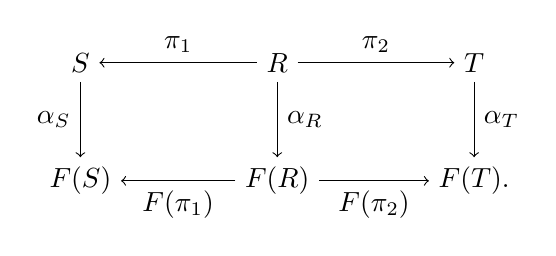
\begin{tikzpicture}
\node[fill=white] (a) at (7.5,0) {$S$};
\node[fill=white] (b) at (10,0) {$R$};
\node[fill=white] (c) at (7.5,-1.5) {$F(S)$};
\node[fill=white] (d) at (10,-1.5) {$F(R)$};
\node[fill=white] (e) at (12.5,0) {$T$};
\node[fill=white] (f) at (12.5,-1.5) {$F(T).$};
\draw[->] (b) to node [above]{$\pi_1$} (a);
\draw[->] (a) to node [left]{$\alpha_S$} (c);
\draw[->] (b) to node [right]{$\alpha_R$} (d);
\draw[->] (d) to node [below]{$F(\pi_1)$} (c);
\draw[->] (b) to node [above]{$\pi_2$} (e);
\draw[->] (e) to node [right]{$\alpha_T$} (f);
\draw[->] (d) to node [below]{$F(\pi_2)$} (f);
\end{tikzpicture}
\end{center}
We say that $s\in S$ and $t\in T$ are $F$-bisimilar, written by $s\sim t$, if they are related by some $F$-bisimulation between $S$ and $T$. There exists another notion of coalgebraic equality from another perspective. Two elements $s$ and $t$ are called behaviorally equivalent if there are a coalgebra $(W,\alpha_W)$ and a cospan of homomorphisms $g:S\rightarrow W$ and $h:T\rightarrow W$:
\begin{center}
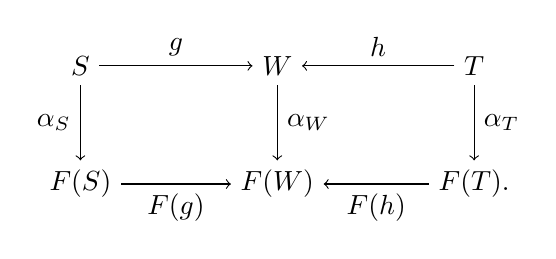
\begin{tikzpicture}
\node[fill=white] (a) at (7.5,0) {$S$};
\node[fill=white] (b) at (10,0) {$W$};
\node[fill=white] (c) at (7.5,-1.5) {$F(S)$};
\node[fill=white] (d) at (10,-1.5) {$F(W)$};
\node[fill=white] (e) at (12.5,0) {$T$};
\node[fill=white] (f) at (12.5,-1.5) {$F(T).$};
\draw[->] (a) to node [above]{$g$} (b);
\draw[->] (a) to node [left]{$\alpha_S$} (c);
\draw[->] (b) to node [right]{$\alpha_W$} (d);
\draw[->] (c) to node [below]{$F(g)$} (d);
\draw[->] (e) to node [above]{$h$} (b);
\draw[->] (e) to node [right]{$\alpha_T$} (f);
\draw[->] (f) to node [below]{$F(h)$} (d);
\end{tikzpicture}
\end{center}
with $h(s)=g(t)$.

Given two functors $F$ and $G$ between the categories $C$ and $D$, a natural transformation $\eta$ from $F$ to $G$ is a family of morphisms, which must associate to every object $X$ in $C$ a morphism $\eta_X:F(X)\rightarrow G(X)$ in $D$, satisfying $\eta_Y\circ F(f)=G(h)\circ \eta_X$ for every morphism $h:X\rightarrow Y$ in $C$. A natural transformation $\eta$ can induced a functor $T_\eta:\textbf{Coalg}_F\rightarrow \textbf{Coalg}_G$ defined as 
$$T_\eta(S,\alpha_S)=(S,\eta_S\circ \alpha_S)\ and\ T_\eta f=f.$$ 
A translation functor is a functor induced by some transformation. Note that translation functors preserve and reflect bisimilarity. A monad is a triple $(T,\eta,\mu)$, where $T$ is an endofunctor on $C$, $\eta:\mathcal{I}\rightarrow T$ and $\mu:T^2\rightarrow T$ are natural transformations satisfying:
$$
\begin{aligned}
\mu\circ T\mu=&\mu\circ \mu T\\
\mu\circ T\eta=&\mu\circ \eta T=\mathcal{I}.
\end{aligned}
$$
We call $\eta$ and $\mu$, respectively, the unit and the multiplication. 


\nevComment{\underline{Goal of this subsection}: To introduce the reader
to Coalgebra. References from subsection 1.2 can be used here.}


\subsection{Coalgebraic analysis of probabilistic systems: an
  illustration of the abstraction power that is provided by coalgebras}
In both probabilistic and quantum systems, states change with probabilistic laws. The difference is that a probability is given as a real number in probabilistic systems but as a complex number in quantum systems. Real number probabilities can only increase when added, while complex numbers can cancel each other and lower their probability. 
  
Before we consider the quantum case, we see how coalgebraic methods can be used for studying and developing different types of probabilistic systems.  A unified framework of probabilistic systems is proposed in \cite{sokolova}. Different types of probabilistic systems are modeled as coalgebras of suitable behavior endofunctors on $\textbf{Sets}$ as the following table:
\[
\begin{tabular}{|c|c|c|}
\hline
$\textbf{Coalg}_F$ & $F$  & name \\ \hline
\textbf{MC} & $\mathcal{D}$ & Markov chains\\ \hline
\textbf{DLTS} & $(\mathcal{I}+1)^A$ & deterministic automata \\ \hline
\textbf{LTS} & $\mathcal{P}(A\times\mathcal{I})\cong\mathcal{P}^A$ & non-deterministic automata \\ \hline
\textbf{React} & $(\mathcal{D}+1)^A$ & reactive systems \\ \hline
\textbf{Gen} & $\mathcal{D}(A\times\mathcal{I})+1$ & generative systems \\ \hline
\textbf{Str} & $\mathcal{D}+(A\times\mathcal{I})+1$ & stratified systems \\ \hline
\textbf{Alt} & $\mathcal{D}+\mathcal{P}(A\times\mathcal{I})$ & alternating systems \\ \hline
\textbf{Var} & $\mathcal{D}(A\times \mathcal{I})\cup\mathcal{P}(A\times\mathcal{I})$ & Vardi systems \\ \hline
\textbf{SSeg} & $\mathcal{P}(A\times \mathcal{D})$ & simple Segala systems \\ \hline
\textbf{Seg} & $\mathcal{PD}(A\times\mathcal{I})$ & Segala systems \\ \hline
\textbf{Bun} & $\mathcal{DP}(A\times\mathcal{I})$ & bundle systems \\ \hline
\textbf{PZ} & $\mathcal{PDP}(A\times\mathcal{I})$ & Pnueli-Zuck systems \\ \hline
\textbf{MG} & $\mathcal{PDP}(A\times\mathcal{I}+\mathcal{I})$ & most general systems\\ \hline
\end{tabular}
\]

$\textbf{Coalg}_F$ is coalgebraically embedded in $\textbf{Coalg}_G$ if there exists a translation functor from $\textbf{Coalg}_F$ to $\textbf{Coalg}_G$, which preserves and reflects bisimilarity. It can be thought that there exists a $G$-coalgebra as a ``copy'' of an $F$-coalgebra if $\textbf{Coalg}_F$ is coalgebraically embedded in $\textbf{Coalg}_G$, and therefore it is considered that $G$-coalgebras are at least as expressive as $F$-coalgebras. There is a hierarchy of probabilistic system types as the following graph:
\begin{center}
\begin{tikzpicture}
\node[fill=white] (a) at (0,0) {\textbf{React}};
\node[fill=white] (b) at (3,0) {\textbf{LTS}};
\node[fill=white] (c) at (6,0) {\textbf{Gen}};
\node[fill=white] (d) at (9,0) {\textbf{Str}};
\node[fill=white] (e) at (1.5,-1.5) {\textbf{DLTS}};
\node[fill=white] (f) at (9,-1.5) {\textbf{MC}};
\node[fill=white] (g) at (1.5,1.5) {\textbf{SSeg}};
\node[fill=white] (h) at (4.5,1.5) {\textbf{Var}};
\node[fill=white] (i) at (9,1.5) {\textbf{Alt}};
\node[fill=white] (j) at (3,3) {\textbf{Seg}};
\node[fill=white] (k) at (6,3) {\textbf{Bun}};
\node[fill=white] (l) at (4.5,4.5) {\textbf{PZ}};
\node[fill=white] (m) at (6,6) {\textbf{MG}};
\draw[->] (a) to (g);
\draw[->] (b) to (g);
\draw[->] (b) to (h);
\draw[->] (c) to (h);
\draw[->] (d) to (i);
\draw[->] (e) to (a);
\draw[->] (e) to (b);
\draw[->] (f) to (d);
\draw[->] (g) to (j);
\draw[->] (h) to (j);
\draw[->] (h) to (k);
\draw[->] (i) to (m);
\draw[->] (j) to (l);
\draw[->] (k) to (l);
\draw[->] (l) to (m);
\end{tikzpicture}
\end{center}
where an arrow $\textbf{A}\rightarrow \textbf{B}$ indicates that $\textbf{A}$ is coalgebracially embeddable in the class $\textbf{B}$.

\nevComment{\underline{Goal of this subsection}: To convince the
  reader that Coalgebra is a powerful abstraction tool for studying
  and developing different types of state-based transition systems.
  This justifies our choice of the coalgebraic approach for
  accomplishing the goals presented above. Our illustration should concern
  probabilistic systems because they are close to quantum ones. The
  main reference for this subsection is \cite{sokolova}.}


\section{Current Formalisms for Quantum transition systems}
In this section we introduce some current formalisms for quantum transition systems, including automata theory and different coalgebraic methods. 

\subsection{Quantum automata}
There exists different versions of quantum automata, such as MM-QFA, MO-QFA, Latvian QFA and so on. Here we introduced the most general QFA model \cite{hirvensalo11,AA14}.
\begin{definition}
A n-state QFA is a quintuple $M=(Q,\Sigma,\delta,q_0,q_F)$, where $Q=\{q_1,\cdots,q_n\}$ is a finite set of states, $\Sigma$ an alphabet, $q_I$ the initial state, $q_F$ the set of final states, and $\delta:\Sigma\rightarrow B(B(H_n))$ a transition function associating to each letter $a\in \Sigma$ a quantum operation over $H_n$. 
\end{definition}
 
The QFA starts in state $\ket{q_I}\bra{q_I}$, and each read input letter changes the state by $V_a=\delta(a):B(H_n)\rightarrow B(H_n)$. Note that $V_{wa}=V_wV_a$. The acceptance probability of the word is given by 
$$f_{M}(w)=Tr(PV_{w^R}\ket{q_I}\bra{q_I}),$$
where $P=\sum_{q\in F}\ket{q}\bra{q}$, $w^R$ is the transpose of $w$ and $Tr(A)$ represents the trace of $A$. 

\begin{example}
We recall Example \ref{QA} and give a specification as a QFA $(\{0,1\},\{a,b\},\delta,\{0\},\{\{0\}\})$, where 
$$
\delta_a(A)=T_aAT_a^*\ and \
\delta_b(A)=T_bAT_b^*.
$$
The probability that the word $ba$ is accepted  is $Tr(\ket{0}\bra{0}T_aT_b\ket{0}\bra{0}T_b^*T_a^*)=\half$. 
\end{example}

\nevComment{\underline{Goal of this subsection}: To introduce the
  reader to quantum automata and related notions. The main reference for this is the
  survey \cite{hirvensalo11}.}

\subsection{Quantum Markov chains}
A Markov chain is a stochastic process to describe a sequence of possible events in which the probability of each event depends only on the state attained in the previous event. Markov chains have many applications as statistical models of real-world processes, which motivates scientists to explore the quantum case of Markov chains \cite{G08,LY15,D18}. As the Example \ref{QRW}, classical quantum Markov chains are specified as triples $(H,\mathcal{E},\phi)$. Here we introduce a different approach based on quantum operations \cite{G08}. 

Given a complex Hilbert space $H$, a transition operation matrix (TOM) is a matrix of the form $\mathcal{E}=[\mathcal{E}_{ij}]$ where $\mathcal{E}_{ij}$ is a completely positive endomap on $\mathcal{B}(H)$ such that $\sum_i\mathcal{E}_{ij}$ is a trace-preserving quantum operation. A quantum Markov chain is a finite or countable directed graph $G$ in which the edge from state $D_j\in \mathcal{DM}(H)$ to state $D_i\in \mathcal{DM}(H)$ is labeled $\mathcal{E}_{ij}$ (if no edge, $\mathcal{E}_{ij}=0$) and $\mathcal{E}=[\mathcal{E}_{ij}]$ forms a TOM. It has been proved that this definition is equivalent to classical counterpart. 

\begin{example}
Recall the Example \ref{QRW}, there exists a corresponding quantum Markov chain for the Hilbert space $H=\mathbb{C}^2\otimes \mathcal{M}(\mathbb{Z})$. The set of states is $$\{(\ket{\uparrow}\otimes\ket{i})(\bra{\uparrow}\otimes\bra{i}),(\ket{\downarrow}\otimes\ket{i})(\bra{\downarrow}\otimes\bra{i})|i\in \mathbb{Z}\}.$$
The TOM $\mathcal{E}=[\mathcal{E}_{ij}]$ is defined as follows:
$$\mathcal{E}_{j+1,j}=\{\ket{\uparrow}\bra{\uparrow}H\otimes I\}, \mathcal{E}_{j-1,j}=\{\ket{\downarrow}\bra{\downarrow}H\otimes I\}$$
where $H$ is the Hadamard matrix and $\mathcal{E}_{ij}=0$ for $i\neq j\pm 1, i,j\in\mathbb{Z}$. 
\end{example}

\subsection{Coalgebras over set-based state spaces}
Here we introduce two monads on \textbf{Sets}: the multiset monad \cite{B11} and the quantum branching monad \cite{hasuo17,ogawa14}. More over, we introduce some applications of them. 

\begin{definition}(multiset monad $\mathcal{M}$)
 The multiset monad $\mathcal{M}:\textbf{Sets}\rightarrow \textbf{Sets}$ is defined as follows:
 $$ 
 \begin{aligned}
 \mathcal{M}(X)&:=\{z_1\ket{x_1}+\dots+z_n\ket{x_n}|z_i\in \mathbb{C} \ and\ x_i\in X\}\\
 \mathcal{M}(f)(z_1&\ket{x_1}+\dots+z_n\ket{x_n}):=z_1\ket{f(x_1)}+\dots+z_n\ket{f(x_n)}.
 \end{aligned}
 $$
 Such a multiset $sum_i z_i\ket{x_i}\in\mathcal{M}(X)$ can equivalently be described as a function $X\rightarrow \mathbb{C}$ with finite support.
 The unit $\eta:X\rightarrow \mathcal{M}(X)$ and the multiplication $\mu:\mathcal{M}^2(X)\rightarrow \mathcal{M}(X)$ are:
 $$
 \begin{aligned}
 \eta_X(x)&:=\{\ket{x}\}\\
 \mu_X(z_1h_1+\dots+z_n h_n)&:=\lambda x\in X. z_1\cdot h_1(x)+\dots+z_n\cdot h_n(x)
 \end{aligned}
 $$
 where the notation $\lambda x\in X.\cdots$ is used for the function $x\mapsto \cdots$.
\end{definition}

\begin{example}
Recall the Example \ref{QRW} and there exist a linear mapping $q:\mathbb{C}^2\otimes\mathcal{M}(\mathbb{Z})\rightarrow \mathbb{C}^2\otimes\mathcal{M}(\mathbb{Z})$ corresponding to the quantum operation:
$$
\begin{aligned}
q:\mathbb{C}^2\otimes\mathcal{M}(\mathbb{Z})&\rightarrow \mathbb{C}^2\otimes\mathcal{M}(\mathbb{Z})\\
\ket{\uparrow}\otimes \ket{i}&\mapsto\roothalf\ket{\uparrow}\otimes\ket{i-1}+\roothalf\ket{\downarrow}\otimes\ket{i+1}\\
\ket{\downarrow}\otimes \ket{i}&\mapsto\roothalf\ket{\uparrow}\otimes\ket{i-1}+\roothalf\ket{\downarrow}\otimes\ket{i+1}
\end{aligned}
$$
Moreover, there exists a coalgebra $\mathbb{Z}\rightarrow \mathcal{M}(\mathbb{Z}+\mathbb{Z})^2$ corresponding to the linear mapping $q:\mathbb{C}^2\otimes\mathcal{M}(\mathbb{Z})\rightarrow \mathbb{C}^2\otimes\mathcal{M}(\mathbb{Z})$, which can be described explicitly as follows. 
$$
\begin{aligned}
\mathbb{Z}&\rightarrow \mathcal{M}(\mathbb{Z}+\mathbb{Z})^2\\
i&\mapsto \langle\roothalf k_1\ket{i-1}+\roothalf k_2\ket{i+1},\roothalf k_1\ket{i-1}-\roothalf k_2{i+1}\rangle
\end{aligned}
$$
where $k_1$ and $k_2$ are coprojections that serve as tags for `left' and `right' in a coproduct $\mathbb{Z}+\mathbb{Z}$. Note that the functor $\mathcal{M}(2\cdot -)^2$ can also induce a monad \cite{B11}. 
\end{example}

\begin{definition}(quantum branching monad)
The quantum branching monad $\mathcal{Q}:\textbf{Sets}\rightarrow \textbf{Sets}$ is defined as follows:
$$
\begin{aligned}
\mathcal{Q}&(X):=\{c:X\rightarrow\prod_{m,n\in\mathbb{N}}QO_{m,n}|\sum_{x\in X}\sum_{n\in\mathbb{N}}\mathbf{tr}((c(x))_{m,n}(\rho))\leq 1,\forall m\in \mathbb{N},\forall\rho\in\mathcal{DM}(H_m).\}\\
(\mathcal{Q}&(f)(c)(y))_{m,n}:=\sum_{x\in f^{-1}(y)}(c(x))_{m,n}
\end{aligned}
$$
where $\prod_{m,n\in\mathbb{N}}$ denotes a Cartesian product and $(c(x))_{m,n}$ is the $(m,n)$-component of $c(x)\in\prod_{i,j}QO_{i,j}$. 
The unit and the multiplication are:
$$
\begin{aligned}
(\eta_X(x)(x'))_{m,n}&:=\begin{cases} \{\mathcal{I}_m\} & \ if\ x=x'\ and\ m=n\\ 0 &\ otherwise \end{cases}\\
(\mu_X(h)(x'))_{m,n}&:=\sum_{c\in\mathcal{Q}(X)}\sum_{k\in\mathbb{N}}((c(x))_{k,n}\circ(h(c))_{m,k})
\end{aligned}
$$
where $\mathcal{I}_m$ is a $m\times m$ identity matrix and 0 is a zero operation which maps any density matrix to zero.
\end{definition}

It is shown that states are $\mathcal{D}$-bisimilar is equal to they are behavioral equivalent in probabilistic systems, where $\mathcal{D}$ is the distribution monad. But it does not hold in the quantum case. There exists an example indicating that two states can be behavioral equivalent but not $\mathcal{Q}$-bisimilar. However, built on the quantum branching monad, quantum labeled transition systems can be defined.  

\begin{definition}(quantum LTS) A QLTS $(X,s,c)$ consists of a set $X$ and a pair of functions $s:1\rightarrow \mathcal{Q}(X)$ and $c:X\rightarrow\mathcal{Q}(1+\Sigma\times X)$, where $\Sigma$ is an alphabet. 
\end{definition}

\begin{example}
Recall the Example \ref{QTP} and there exist a corresponding QLTS (when $\Sigma=\{\tau\}$) $(X,s:\mathcal{Q}(X),c:X\rightarrow \mathcal{Q}(1+X))$:
$$
\begin{aligned}
X&=\{x_0,x_{00},x_{01},x_{10},x_{11},\surd\}\\
(s(x_0))_{2,8}&=\lambda\rho\in\mathcal{DM}(H_2).\rho\otimes\ket{\Phi^+}\bra{\Phi^+}\\
(c(x_0)(x_i))_{8,2}&=
\begin{cases}
\{(\bra{\Phi^+}\otimes\mathcal{I}_2)\}\ \ \ if\ i=00\\ 
\{(\bra{\Phi^-}\otimes\mathcal{I}_2)\}\ \ \ if\ i=01\\ 
\{(\bra{\Psi^+}\otimes\mathcal{I}_2)\}\ \ \ if\ i=10\\ 
\{(\bra{\Psi^-}\otimes\mathcal{I}_2)\}\ \ \ if\ i=11
\end{cases}\\
(c(x_i)(\surd))_{2,2}&=
\begin{cases}
\{\mathcal{I}_2\}\ &if\ i=00\\
\{X\}\ &if\ i=01\\
\{Z\}\ &if\ i=10\\
\{ZX\}\ &if\ i=11
\end{cases}
\end{aligned}
$$
\end{example}

\nevComment{\underline{Goal of this subsection}: To introduce the
reader to Ichiro's and Ogawa's formalism (which involves the quantum
branching monad) \cite{hasuo17,ogawa14}. The notions of behavioral
equivalence proposed in these two references should also be mentioned, as they are one
clear source of motivation to our goals.}

\subsection{Coalgebras over Hilbert-based state spaces}
In the category \textbf{Sets}, the features of quantum states are not explicit. When we focus on the set of mixed states (density matrices) of a n-level quantum system, it is easy to find that $\mathcal{DM}(H_n)$ is a convex set. There exists a coalgebraic model for quantum systems based on the category \textbf{Conv} in \cite{F14}.

Consider the endofunctor $F(X)=[0,1]^E\times X^S$ on the category \textbf{Conv}, a Hilbert space $H$, a set $E$ of some effects and a set $S$ of some trace-preserving quantum operations, which can be represented by $\{U\}$ where $U$ is unitary. Form the $F$-coalgebra
$$
\begin{aligned}
f:\mathcal{DM}(H)&\rightarrow[0,1]^E\times \mathcal{DM}(H)^S\\
\rho&\mapsto((\mathbf{tr}(\rho\epsilon))_{\epsilon\in E},(U\rho U^*)_U\in S). 
\end{aligned}
$$
The part $\mathbf{tr}(\rho\epsilon)$ is the probability that measurement of the effect $\epsilon$ succeeds when the system is in mixed state $\rho$. 

\begin{example}
\label{CQA}
Recall the Example \ref{QA} and there exists a corresponding $F$-coalgebra:
$$
\begin{aligned}
\mathcal{DM}(\mathbb{C}^2)&\rightarrow [0,1]\times \mathcal{DM}(\mathbb{C}^2)^{\{a,b\}}\\
\rho&\mapsto(\mathbf{tr}(\rho\epsilon),(T_r\rho T_r^*)_{r\in \{a,b\}}).
\end{aligned}
$$ 
\end{example}

\begin{example}
Recall the Example \ref{QRW} and there exists a corresponding $F$-coalgebra:
$$
\begin{aligned}
\mathcal{DM}(\mathbb{C}^2\otimes\mathcal{M}(\mathbb{Z}))&\rightarrow [0,1]^\mathbb{Z}\times\mathcal{DM}(\mathbb{C}^2\otimes\mathcal{M}(\mathbb{Z}))\\
\rho&\mapsto((\mathbf{tr}(\rho(\ket{\uparrow}\otimes\ket{i})(\bra{\uparrow}\otimes\bra{i})+\rho(\ket{\downarrow}\otimes\ket{i})(\bra{\downarrow}\otimes\bra{i}))_{i\in\mathbb{Z}},\mathcal{E}\rho\mathcal{E}^*).
\end{aligned}
$$
\end{example}

It should be mentioned the coalgebraic perspective on minimization, which is relevant in many areas of computer science such as model checking, concurrency theory, language theory and formal verification \cite{JFMBSA12}. In general terms, a minimal coalgebra is the coalgebra with the smallest state space among those with the same behavior and the notion of minimization is to find a minimal coalgebra. An interesting thing if that for the functor $F(X)=[0,1]^E\times X^S$ the minimal coalgebra with the behavior $b:1\rightarrow ([0,1]^E)^{S^*}$ need not be a quantum coalgebra, even if the behavior arises from a quantum system. The minimal coalgebra can be regarded as a probabilistic system, whose state space is not necessarily of the form $\mathcal{DM}(H)$. 

In quantum mechanics, the Heisenberg picture is a formulation in which the operators change by time, but the states are time-independent. In contrast, the Sch$\ddot{o}$dinger picture is a formulation in which the operators are constant but the states evolve  in time. The two pictures  have been proved equivalent by physical methods. It is easy to find an $F$-coalgebra corresponds to a Sch$\ddot{o}$dinger, which provides a coalgebraic perspective to model the Heisenberg picture as another shape of coalgebras and  prove the equivalence between the two shapes of coalgebras by generalized duality, which can also be used applied to other functors and categories. 

\nevComment{\underline{Goal of this subsection}: To introduce the
  reader to Roumen's formalism \cite{F14}. The notions of minimisation
  that were proposed and the duality between Schrodinger and Heisenberg should
  also be mentioned; for the same reason than above.}


\section{Relation between formalisms of quantum transition systems}

\subsection{A uniform view of quantum transition systems}

\nevComment{\underline{Goal of this subsection}: To provide the reader with a uniform
view of quantum automata \cite{hirvensalo11} using a coalgebraic approach. Extend this
view to Ichiro's and Roumen's coalgebras if possible; and if not explain why.}

\subsection{A hierarchy of formalisms for quantum transition systems}
Given a coalgebraic model $$\mathcal{DM}(H)\rightarrow [0,1]^{E}\times \mathcal{DM}(H)^{S}$$
where $dim(H)=n$, $E=\{\epsilon_{1},\dots,\epsilon_{e}\}$ and $S=\{U_1,\dots,U_s\}$, define $X=\{x_0,x_1,\dots,x_s,y_1,\dots,y_e\}$ and the corresponding QLTS $(X,s,c)$ as follows:
$$
\begin{aligned}
(s(x_0))_{n,n}&=\lambda \rho\in \mathcal{DM}(H_n). \rho\\
(c(x_i)(x_j))_{n,n}&=\{U_j\}\ \ \ i=0,1,\dots,s\ and\ j=1,\dots,s\\
(c(x_i)(y_j))_{n,n}(\rho)&=\rho \epsilon_{j}\ \ \ \ \ i=0,1,\dots,s\ and\ j=1,\dots,e\\
(c(y_i)(\surd))_{n,n}&=\{I_n\}\ \ \ i=1,\dots,e
\end{aligned}
$$

\begin{example}
Recall  the Example \ref{CQA} and the corresponding $F$-coalgebra gives a QLTS $(X,s,c)$ with the initial state $\ket{0}\bra{0}$, where $X=\{x_0,x_1,x_2,y\}$ and 
$$
\begin{aligned}
(s(x_0))_{2,2}&=\lambda \rho\in \mathcal{DM}(\mathbb{C}^{2}). \rho\\
(c(x_i)(x_j))_{2,2}&=\begin{cases}
\{\delta_a\} &j=1\\
\{\delta_b\} &j=2
\end{cases},\ i=0,1,2\\
(c(x_i)(y))_{2,2}(\rho)&=\rho \epsilon,\ i=0,1,2\\
(c(y)(\surd))_{2,2}&=\{I_2\}.
\end{aligned}
$$


\end{example}



\nevComment{\underline{Goal of this subsection}: Establish a hierarchy
  of formalisms for quantum transition systems. In the coalgebraic
  approach this ammounts to having monomorphic natural transformations
  between the functors of interest (see \cite[Section 4.4]{sokolova}).
}

\section{Summary}

\nevComment{\underline{Goal of this subsection}: To give a broad
  picture of the results achieved in the previous section. In
  particular, a diagram depicting the hierarchy established, and the
  (dis)advantages of each formalism. At the end of this section, the
  reader should have,
  \begin{enumerate}
  \item a clear overview of existing formalisms for quantum transition systems,
  \item and how they relate to each other in terms of expressivity,
  \item a clear understanding of which formalism to choose for modelling a certain quantum
    system,
  \item and a coalgebraic definition that captures all different
    notions of quantum transition system.
  \end{enumerate}
  The reader should be convinced that the paper gave him enough tools to be able to study and develop
  useful notions for quantum transitions systems \underline{in a uniform manner}. 
}

\noindent
\nevComment{{\large \underline{Deadline}: 10th of October 2018.}}


\section{\dots}

\subsection*{Acknowledgement}
\noindent The work was partially supported by the National Natural Science Foundation of China under grant no. 61772038, 61532019, 61202069 and 61272160.

%%Bibliography
\bibliographystyle{alpha}
\bibliography{the}

\end{document}